\documentclass[12pt, leqno]{article} %% use to set typesize
\input{common}

\usepackage{fontspec}
\usepackage{polyglossia}
\setmonofont{DejaVu Sans Mono}[Scale=MatchLowercase]
\usepackage[outputdir=pdf]{minted}

\providecommand{\tightlist}{%
  \setlength{\itemsep}{0pt}\setlength{\parskip}{0pt}}
\begin{document}



\hdr{2023-04-17}

\section{Broadening the Basin}

All the methods we have so far discussed for solving nonlinear equations
or optimization problems have the form \[x_{k+1} = x_k + \alpha_k p_k\]
where \(\alpha_k\) is a \emph{step size} and \(p_k\) is a \emph{search
direction}. We have described a wide variety of methods for choosing the
search directions \(p_k\). We have also analyzed several of these
methods (or at least pointed to their analysis) under the assumption
that the step sizes were chosen to be \(\alpha_k = 1\) (or, in our
analysis of gradient descent, \(\alpha_k = \alpha\) some constant). But
so far, our analyses have all come with the caveat that convergence is
only assured for initial guesses that are ``good enough.'' We call the
set of initial guesses for which a nonlinear solver or optimizer
converges to a given solution \(x_*\) the \emph{basin of convergence}
for \(x_*\). In a previous lecture, we have already discussed some
features that make the basin of convergence large or small for Newton
and modified Newton iterations. Today we begin our discussion of
\emph{globalization} methods that allow us to guarantee convergence even
if we lack a good enough initial guess to make our unguarded iterations
converge.

In our discussion today, it will be convenient to focus on globalization
by \emph{line search methods} that make intelligent, adaptive choices of
the step size. Informally, these methods work with any ``reasonable''
method for choosing search directions \(p_k\) (which should at least be
descent directions). An \emph{exact line search} method seeks to
minimize \(g(\alpha) = \phi(x_k + \alpha p_k)\) by a one-dimensional
optimization; but it turns out that the work required for exact line
search usually does not justify the benefit. Instead, we consider
\emph{inexact line search} methods that choose step sizes \(\alpha_k\)
such that the methods:

\begin{itemize}
\tightlist
\item
  Make significant progress in the downhill direction (\(\alpha_k\) not
  too small).
\item
  But don't step so far they go back uphill (\(\alpha_k\) not too big).
\end{itemize}

We need to tighten and formalize these conditions a little bit in order
to obtain formal convergence results, but this is the right intuition.

\section{A series of unfortunate examples}

In order to illustrate the conditions we will require -- and the limits
of our approach -- we will first consider three illustrative examples.

\subsection{The long march to infinity}

Consider the one-dimensional objective function
\[\phi(x) = x \tan^{-1}(x) - \frac{1}{2} \log(1+x^2).\] The first and
second derivatives of \(\phi\) are \begin{align*}
  \phi'(x) &= \tan^{-1}(x) \\
  \phi''(x) &= \frac{1}{1+x^2}.
\end{align*}

\begin{figure}
\begin{center}
  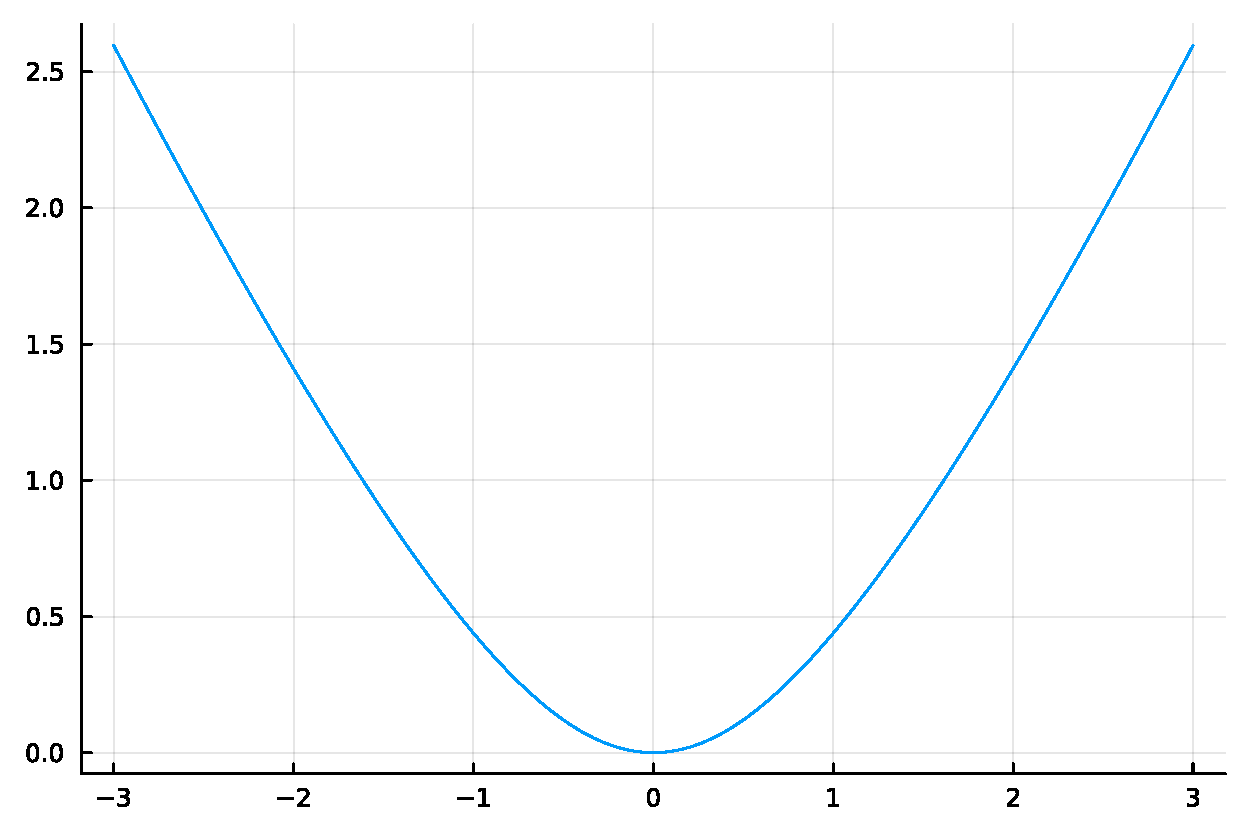
\includegraphics[width=0.8\textwidth]{fig/2023-04-17-phi1.pdf}
\end{center}
\caption{Example function $\phi_1(x)$}
\label{fig:phi1}
\end{figure}

This is a convex function with a unique global 
minimum $\phi(0) = 0$ (Figure~\ref{fig:phi1}).
To find this minimum, we might first consider Newton’s iteration:
\[
  x_{k+1} = x_k - \frac{\phi'(x)}{\phi''(x)} = x_k - (1+x_k^2) \tan^{-1}(x_k).
\]

\begin{figure}
\begin{center}
  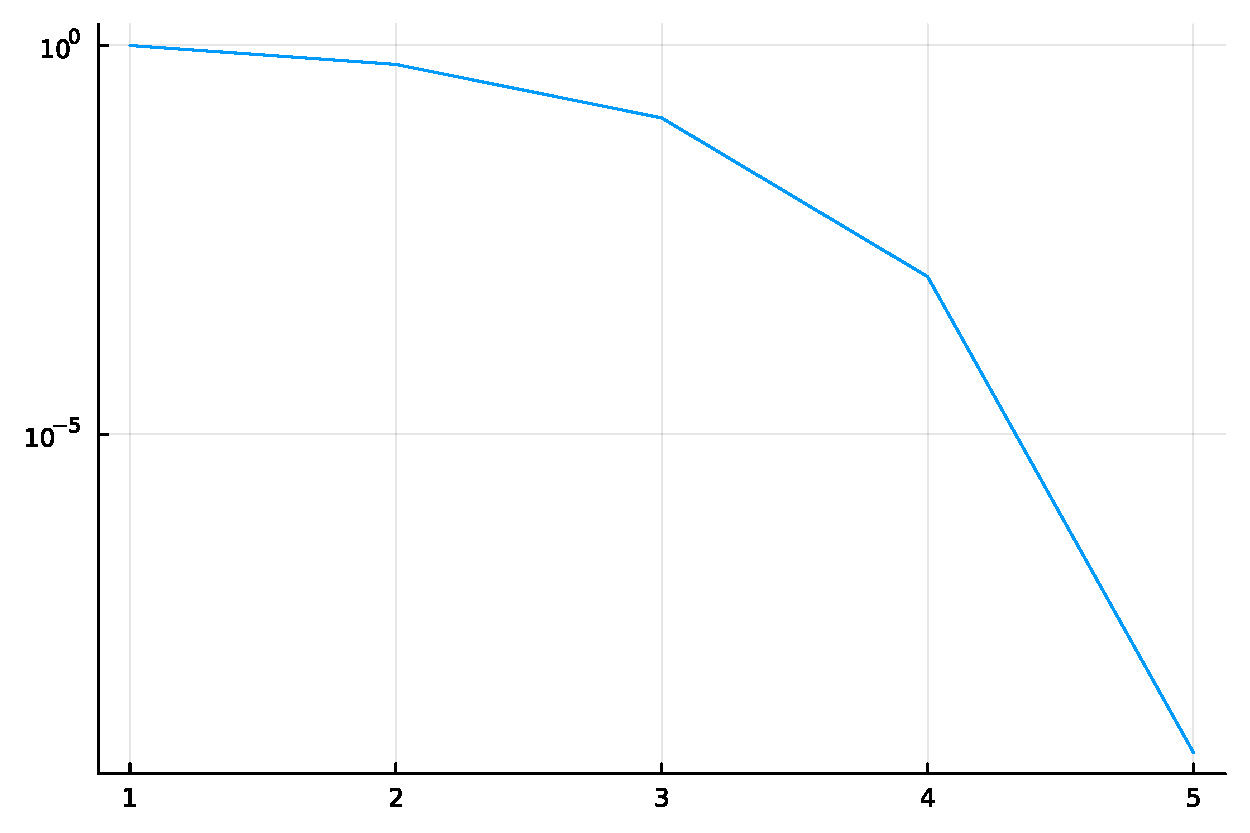
\includegraphics[width=0.8\textwidth]{fig/2023-04-17-phi1-newton0.pdf}
\end{center}
\caption{Convergence of unguarded Newton on $\phi_1(x)$ with $x_0 = 1$}
\label{fig:phi1-newton0}
\end{figure}

The Newton step is always in a descent direction, and the iteration
converges for \(|x_0| \leq \xi \approx 1.3917\); here \(\xi\) is the
solution to the ``anti-fixed-point'' equation
\[-\xi = \xi - (1+\xi^2) \tan^{-1}(\xi).\]

\begin{figure}
\begin{center}
  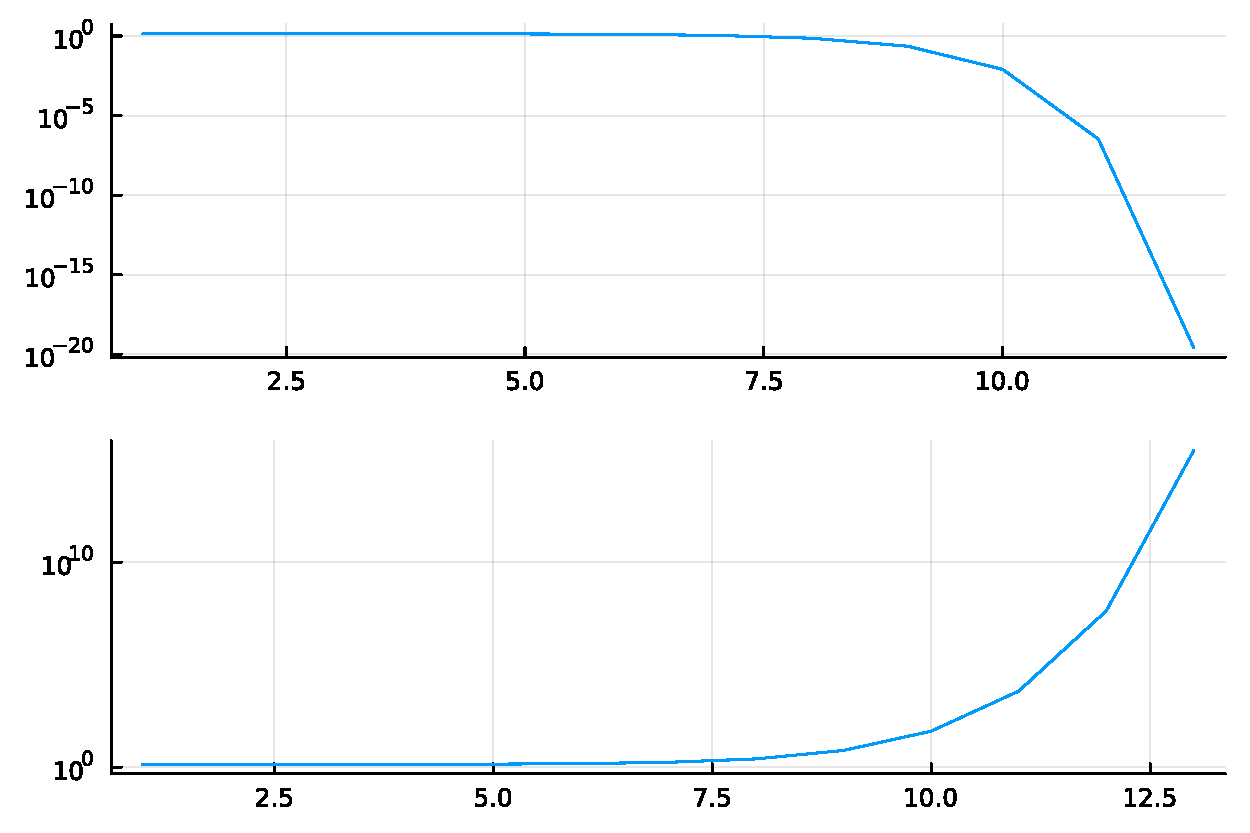
\includegraphics[width=0.8\textwidth]{fig/2023-04-17-phi1-newton12.pdf}
\end{center}
\caption{Convergence of unguarded Newton on $\phi_1(x)$ with $x_0 = \xi \mp 10^{-3}$}
\label{fig:phi1-newton12}
\end{figure}

For any $|x_0| < \xi$, the iterates monotonically decrease in magnitude,
For any $|x_0| > \xi$, the iterates blow up, alternating between 
positive and negative numbers of increasingly wild 
magnitudes (Figure~\ref{fig:phi1-newton12}).
The Newton step always goes in the right direction, but it goes too far.

\begin{minted}{julia}
function backtracking_newton1(x, ϕ, dϕ, Hϕ; nsteps=100, atol=1e-8,
                              monitor=(x, α)->nothing)

    α = 1.0
    p = -dϕ(x)/Hϕ(x)
    
    for k = 1:nsteps
        xnew = x+α*p
        if ϕ(xnew) < ϕ(x)  # Progress!

            # Accept the step
            monitor(x, α)
            x = xnew

            # Check for convergence
            if norm(p) < atol
                return x
            end
            
            # Reset step length and recompute Newton step
            α = 1.
            p = -dϕ(x)/Hϕ(x)

        else  # Step did not decrease ϕ

            # Try with half a step
            α /= 2

        end
    end
    error("Did not converge in $nsteps steps")
end
\end{minted}

\begin{figure}
\begin{center}
  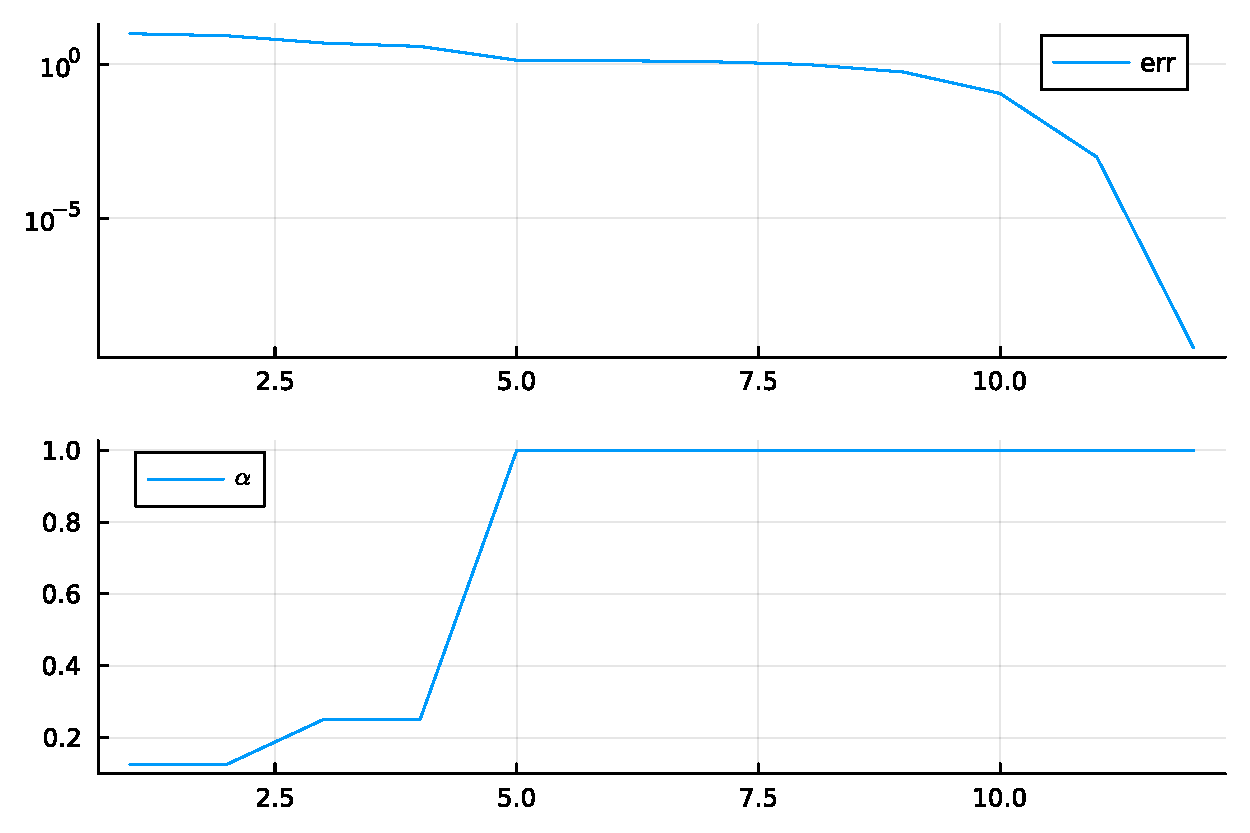
\includegraphics[width=0.8\textwidth]{fig/2023-04-17-phi1-newton-bt.pdf}
\end{center}
\caption{Convergence of simple backtracking Newton on $\phi_1(x)$ with $x_0 = 10$}
\label{fig:phi1-newton-bt}
\end{figure}

We show convergence with simple backtracking in Figure~\ref{fig:phi1-newton-bt}.

\subsubsection{Questions}

\begin{enumerate}
\def\labelenumi{\arabic{enumi}.}
\tightlist
\item
  Where did the equation for \(\xi\) come from?
\item
  Write a monitor function to verify that \(\alpha = 1\) in the call to
  backtracking Newton on this problem iff \(|x| < \xi\).
\end{enumerate}

\subsection{Obscure oscillation}

As a second example, consider minimizing the polynomial
\[\phi(x) = 19x^2 - 4x^4 + \frac{7}{9} x^6.\] The relevant derivatives
are \begin{align*}
  \phi'(x) &= 38x - 16x^3 + \frac{14}{3} x^5 \\
  \phi''(x) &= 38 - 48x^2 + \frac{70}{3} x^4.
\end{align*}

\begin{figure}
\begin{center}
  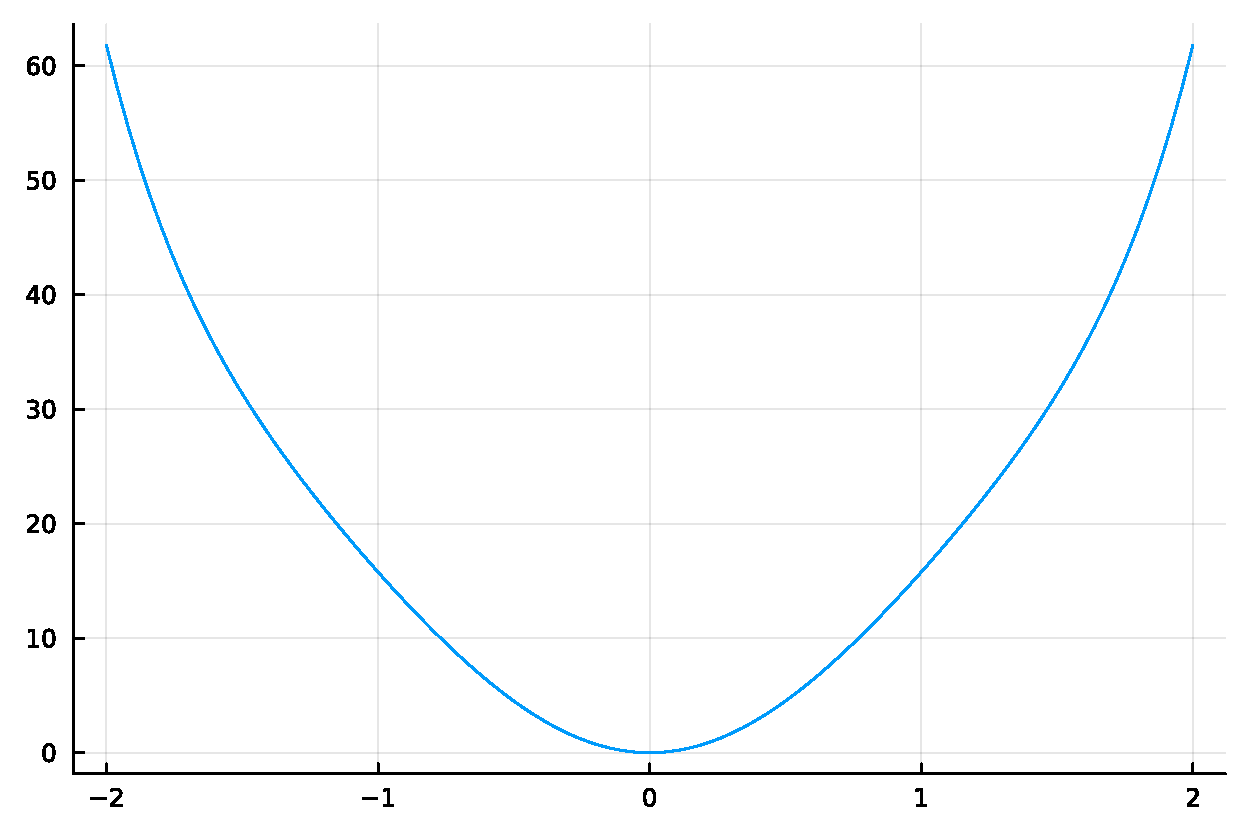
\includegraphics[width=0.8\textwidth]{fig/2023-04-17-phi2.pdf} \\
\end{center}
\caption{Second test function $\phi_2(x)$.}
\label{fig:phi2}
\end{figure}
We show $\phi_2(x)$ in Figure~\ref{fig:phi2}.

The function is convex --- the minimum value of \(\phi''(x)\) is about
\(13.3\) --- and there is a unique global minimum at zero. So what
happens if we start Newton's iteration at \(x_0 = 1.01\)?

\begin{figure}
\begin{center}
  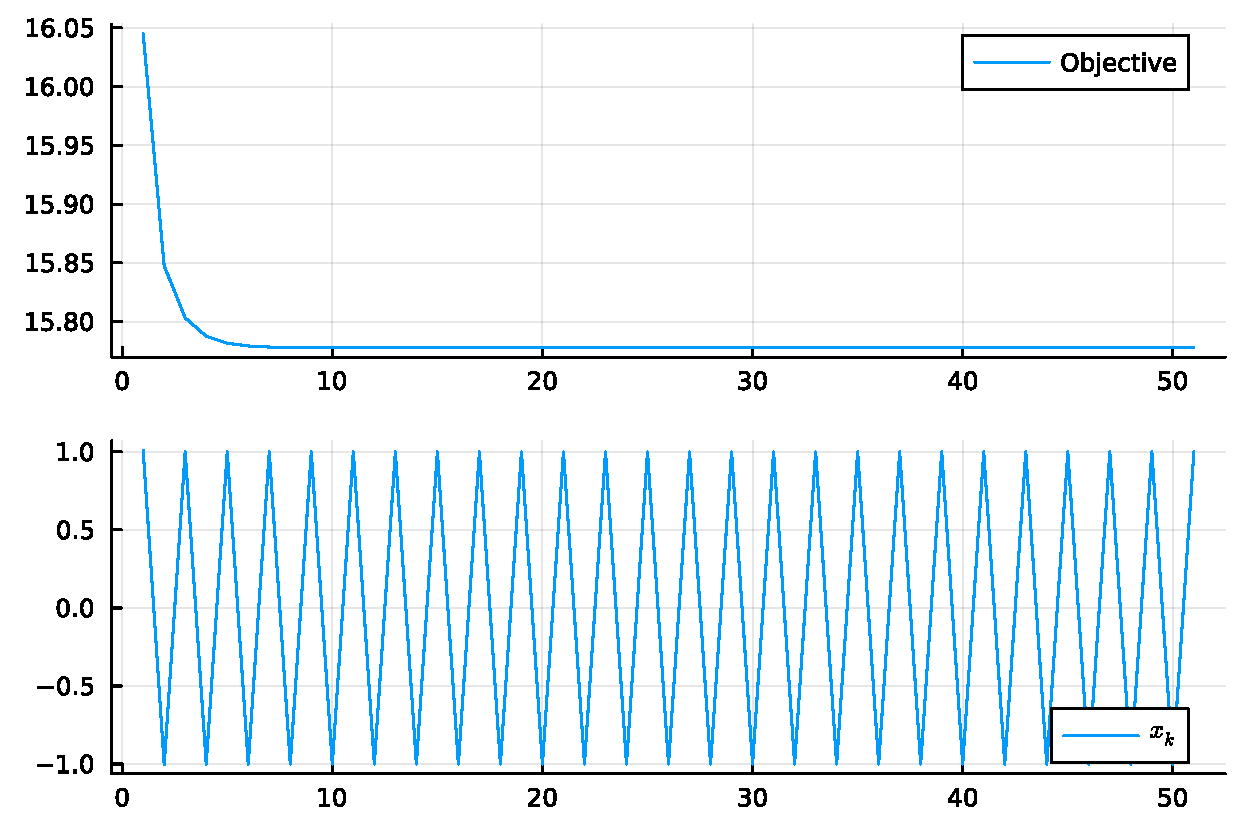
\includegraphics[width=0.8\textwidth]{fig/2023-04-17-phi2-newton.pdf} \\
\end{center}
\caption{Cycling of Newton on $\phi_2(x)$.}
\label{fig:phi2-newton}
\end{figure}

If we look only at the objective values, we seem to be making progress;
each successive iterates is smaller than the preceding one. But the
values of $\phi$ are not converging toward zero, but toward
$\phi(\pm 1) = 142/9 \approx 15.778$! The iterates themselves slosh back
and forth, converging to a limit cycle where the iteration cycles
between $1$ and $-1$ (Figure~\ref{fig:phi2-newton}).

Furthermore, while this polynomial was carefully chosen, the qualitative
cycling behavior is robust to small perturbations to the starting guess
and to the polynomial coefficients. Though it appears to be making
progress, the iteration is well and truly stuck.

The moral is that decreasing the function value from step to step is not
sufficient. Though just insisting on a decrease in the objective
function from step to step will give convergence for many problems, we
need a stronger condition to give any sort of guarantee. But this, too,
can be fixed.

\subsubsection{Questions}

\begin{enumerate}
\def\labelenumi{\arabic{enumi}.}
\tightlist
\item
  Plot \(|\phi(x)-\phi(1)|\) and \(|x|-1\) on a semilog scale for the
  above example. What can you say about the convergence?
\item
  For a general \(\phi\), give a system of two equations in two unknowns
  that characterizes this type of period-2 cycling in Newton iteration.
  For the polynomial in this section, illustrate quadratic convergence
  of a Newton iteration on the equation for the cycle.
\end{enumerate}

\subsection{The planes of despair}

\begin{figure}
\begin{center}
  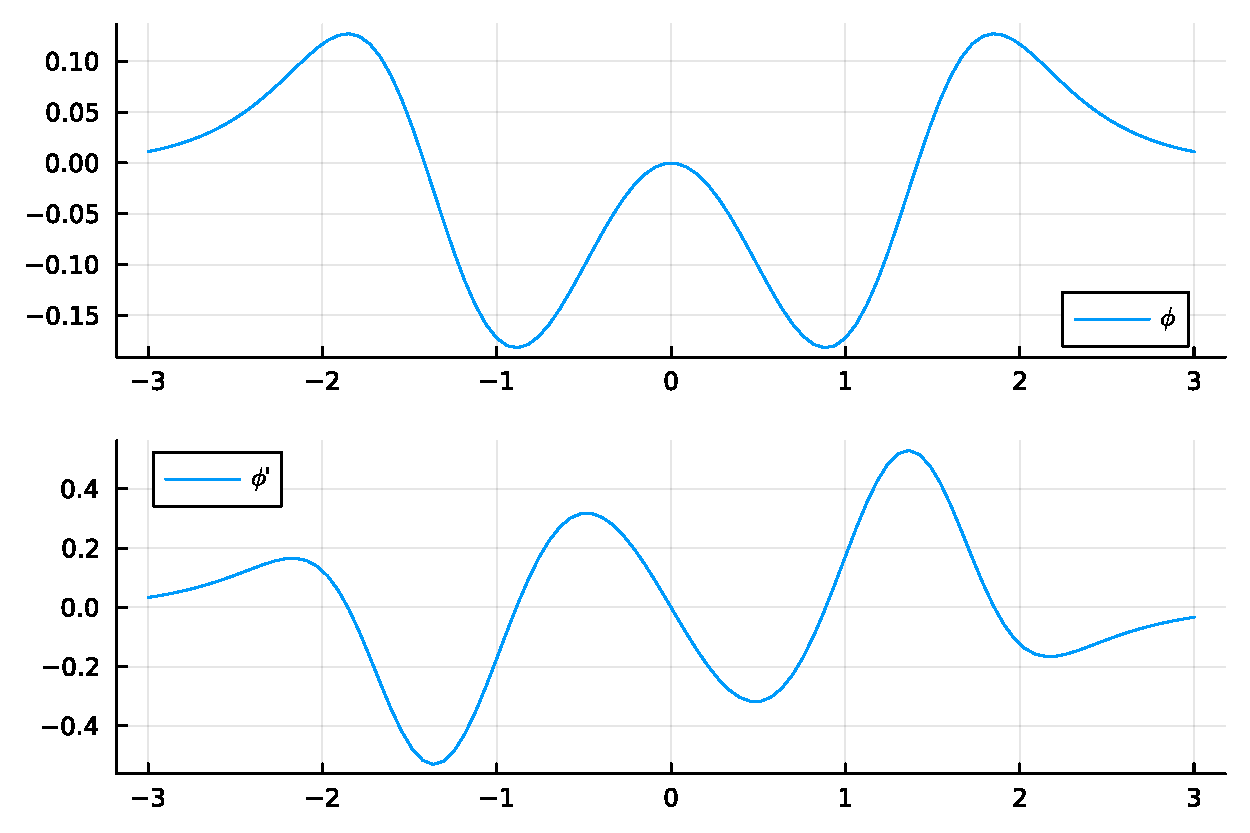
\includegraphics[width=0.8\textwidth]{fig/2023-04-17-phi3.pdf} \\
\end{center}
\caption{Third test function $\phi_3(x)$.}
\label{fig:phi3}
\end{figure}

As a final example, consider the function shown in Figure~\ref{fig:phi3}:
\[
  \phi(x) = \exp(-x^2/2)-\exp(-x^4/4).
\]

This function has two global minima close at around \(\pm 0.88749\)
separated by a local maximum at zero, and two global maximum around
\(\pm 1.8539\). But if we always move in a descent direction, then any
iterate that lands outside the interval \([-1.8539, 1.8539]\) dooms the
iteration to never enter that interval, and hence never find either of
the minima. Instead, most solvers are likely to march off toward
infinity until the function is flat enough that the solver decides it
has converged and terminates. This is the type of problem that we do
\emph{not} solve with globalization, and illustrates why good initial
guesses remain important even with globalization.

\subsubsection{Questions}

\begin{enumerate}
\def\labelenumi{\arabic{enumi}.}
\tightlist
\item
  What does a Newton solver with simple backtracking (as above) do if
  started at \(x = 0\) for this function?
\end{enumerate}

\section{Backtracking search and the Armijo rule}

The idea of a backtracking search is to try successively shorter steps
until reaching one that makes ``good enough'' progress. The step sizes
have the form \(\alpha \rho^j\) for \(j = 0, 1, 2, \ldots\) where
\(\alpha\) is the default step size and \(\rho < 1\) is a backtracking
factor (often chosen to be \(0.5\)). As we saw in our examples, we need
a more stringent acceptance condition than just a decrease in the
function value --- otherwise, we might get unlucky and end up converging
to a limit cycle. That stronger condition is known as the
\emph{sufficient decrease} or the \emph{Armijo rule}. For optimization,
this condition takes the form
\[\phi(x_k + \alpha p_k) \leq \phi(x_k) + c_1 \alpha \phi'(x_k) p_k\]
for some \(c_1 \in (0,1)\). Assuming that \(p_k\) is a descent
direction, this condition can always be satisfied for small enough
\(\alpha\), as Taylor expansion gives
\[\phi(x_k + \alpha p_k) = \phi(x_k) + \alpha \phi'(x_k) p_k + o(\alpha).\]
In practice, it is fine to choose \(c_1\) to be quite small; the value
of \(10^{-4}\) is suggested by several authors. This condition can
always be satisfied for small enough choices of \(\alpha\). Such a line
search algorithm looks much the same as the naive line search that we
described earlier, but with a more complicated termination condition on
the line search loop. The contraction factor \(\rho\) may be chosen a
priori (e.g.~\(\rho = 0.5\)), or it may be chosen dynamically from some
range \([\rho_{\min}, \rho_{\max}]\) where
\(0 < \rho_{\min} < \rho_{\max} < 1\).

\begin{minted}{julia}
function backtracking_newton2(x, ϕ, dϕ, Hϕ; nsteps=100, atol=1e-8,
                              monitor=(x, α)->nothing)

    α = 1.0
    p = -dϕ(x)/Hϕ(x)
    c1 = 1e-4
    
    for k = 1:nsteps
        xnew = x+α*p
 
        # Check sufficient progress (per Armijo)!        
        if ϕ(xnew) <= ϕ(x) + c1*α*dot(dϕ(x), p)  

            # Accept the step
            monitor(x, α)
            x = xnew

            # Check for convergence
            if norm(p) < atol
                return x
            end
            
            # Reset step length and recompute Newton step
            α = 1.
            p = -dϕ(x)/Hϕ(x)

        else  # Step did not decrease ϕ

            # Try with half a step
            α /= 2

        end
    end
    error("Did not converge in $nsteps steps")
end
\end{minted}

\begin{figure}
\begin{center}
  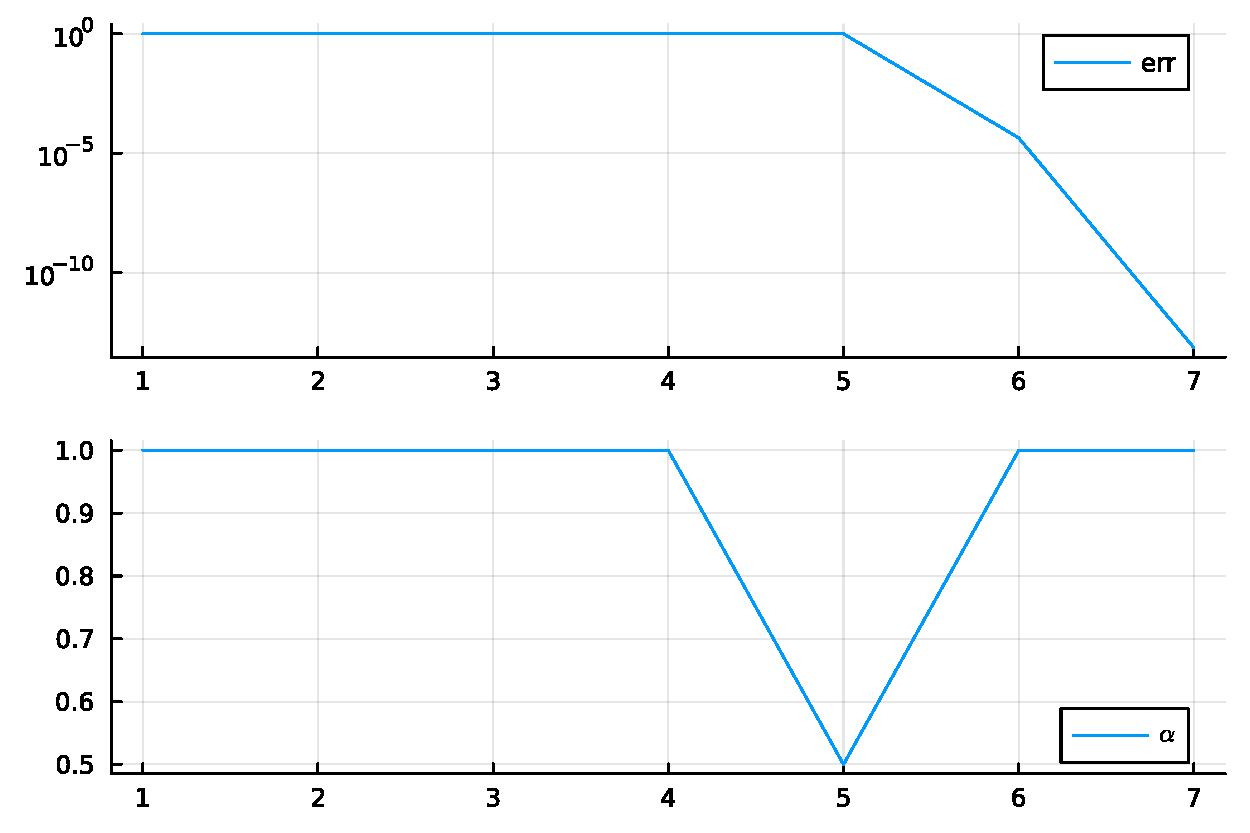
\includegraphics[width=0.8\textwidth]{fig/2023-04-17-phi2-newton-bt.pdf} \\
\end{center}
\caption{Convergence of backtracking Newton on $\phi_2(x)$.}
\label{fig:phi2-newton-bt}
\end{figure}

\section{The curvature condition}

Backtracking line search is not the only way to choose the step length.
For example, one can also use methods based on a polynomial
approximation to the objective function along the ray defined by the
search direction, and this may be a better choice for non-Newton. In
this case, we need to guard not only against steps that are too long,
but also steps that are too short. To do this, it is helpful to enforce
the \emph{curvature condition}
\[\frac{\partial \phi}{\partial p_k}(x_k+\alpha p_k) \geq c_2
  \frac{\partial \phi}{\partial p_k}(x_k)\] for some
\(0 < c_1 < c_2 < 1\). The curvature condition simply says that if the
slope in the \(p_k\) direction at a proposed new point is almost the
same as the slope at the starting point, then we should keep going
downhill! Together, the sufficient descent condition and the curvature
conditions are known as the \emph{Wolfe conditions}. Assuming \(\phi\)
is at least continuously differentiable and that it is bounded from
below along the ray \(x_k+\alpha p_k\), it is always possible to choose
a step size \(\alpha\) that satisfies the Wolfe conditions.

\section{Armijo and nonlinear equations}

While the Armijo rule evolved in optimization theory, the same concept
of sufficient decrease of the function applies in nonlinear equation
solving. To measure progress, we typically monitor the residual norm
\(\|f(x)\|\). If \(p_k = -f'(x_k)^{-1} f(x_k)\) is the Newton direction
from a point \(x_k\), a linear model of \(f\) predicts that
\[\|f(x_k + \alpha p_k)\| \approx
  \|f(x_k) + \alpha f'(x_k) p_k\| =
  (1-\alpha) \|f(x_k)\|;\] that is, the predicted decrease is by
\(\alpha \|f(x_k)\|\). We insist on some fraction of the predicted
decrease as a sufficient decrease to accept a step, yielding the
condition \[\|f(x_k + \alpha p_k)\| \leq (1-c_1 \alpha) \|f(x_k)\|.\] We
don't have to take a Newton step to use this criteria; it is sufficient
that the step satisfy an inexact Newton criterion such as
\[\|f(x_k) + f'(x_k) p_k\| \leq \eta \|f(x_k)\|\] for some \(\eta < 1\).

\section{Global convergence}

In general, if we seek to minimize an objective \(\phi\) that is \(C^1\)
with a Lipschitz first derivative and

\begin{itemize}
\tightlist
\item
  We use one of the line search algorithms sketched above (backtracking
  line search or line search satisfying the Wolfe conditions),
\item
  The steps \(p_k\) are \emph{gradient related}
  (\(\|p_k\| \geq m \|\nabla \phi(x_k)\|\) for all \(k\) -- they don't
  shrink too fast),
\item
  The angles between \(p_k\) and \(-\nabla \phi(x_k)\) are acute and
  uniformly bounded away from away from ninety degrees.
\item
  The iterates are bounded (it is sufficient that the set of points less
  than \(\phi(x_0)\) is bounded),
\end{itemize}

then we are guaranteed global convergence to a stationary point. Of
course, even with all these conditions, we might converge to a saddle or
a local minimizer that is different from the solution we hoped to find;
and we are not guaranteed \emph{fast} convergence. So the choice of
initial guess, and the choice of iterative methods, still matters a
great deal. Nonetheless, the point remains that an appropriately chosen
line search can help improve the convergence behavior of the methods we
have described so far by quite a bit.

We have not described the full range of possible line searches. In
addition to algorithms that inexactly minimize the objective with espect
to the line search parameter, there has also been some work on
\emph{non-monotone} line search algorithms that allow increases in the
function values, as long as progress is made in some more averaged sense
(e.g.~the new point has a objective function value smaller than the
maximum objective function for the past few points). This is useful for
improving convergence speed on some hard problems, and is useful in the
context of particular classes of methods such as spectral projected
gradient (about which we will say nothing in this class other than the
name).


\end{document}
